\documentclass[twoside,a4paper]{book}

\usepackage{lipsum}

\usepackage[pdftex]{graphicx}
\usepackage{wrapfig}
\graphicspath{ {./img/} }
\usepackage[font=small,labelfont=bf]{caption}
\usepackage{amsmath}
\usepackage{amssymb}
\usepackage{textcomp}
\usepackage[utf8]{inputenc}
\usepackage[polish]{babel}
\usepackage[T1]{fontenc}
\usepackage{array}
\usepackage{geometry}
\usepackage{multicol}
% pakiet stosowany do url'i w bibliografii, zamienia odnośniki na ładnie sformatowane
\usepackage{url}
% pakiety służące do numerowania i tworzenia algorytmów
\usepackage{algorithmic}
\usepackage{algorithm}
% redefinicja etykiety nagłówkowej listy algorytmów, domyślna jest po angielsku
\renewcommand{\listalgorithmname}{Spis algorytmów}

% pakiet do wyliczania skali, przydatny przy dużych obrazkach
\usepackage{pgf}
% pakiet służący do automatycznego sortowania odnośników do bibliografii
\usepackage[sort]{natbib}
% tworzenie listingów
\usepackage{listings}
% tworzenie figur wewnątrz figur
\usepackage{subfig}
% do automatycznego skracania nazw rozdziałów i podrozdziałów używanych w nagłówkach strony by mieściły się w jednej linii
\usepackage[fit]{truncate}
% fancyhdr - ładne nagłówki, definicja wyglądu nagłówka, numery stron będą umieszczane w nagłówku po odpowiedniej stronie
\usepackage{fancyhdr}
\pagestyle{fancy}

\renewcommand{\chaptermark}[1]{\markboth{#1}{}}
\renewcommand{\sectionmark}[1]{\markright{\thesection\ #1}}
\fancyhf{}
\fancyhead[LE,RO]{\bfseries\thepage}
% tutaj ograniczamy szerokość pola w nagłówku zawierającego nazwę rozdziału/podrozdziału do 95% szerokości strony
% redefinicja sposobu prezentacji nazw domyślnie wypisywanych wielkimi literami (np. domyślnie w nagłówku Spis treści będzie miał postać SPIS TREŚCI)
% Uwaga! to może popsuć wielkie litery w ogóle! Jak coś nie działa należy usunąć \nouppercase{} z poniższych definicji
\fancyhead[LO]{\nouppercase{\bfseries{\truncate{.95\headwidth}{\rightmark}}}}
\fancyhead[RE]{\nouppercase{\bfseries{\truncate{.95\headwidth}{\leftmark}}}}
\renewcommand{\headrulewidth}{0.5pt}
\renewcommand{\footrulewidth}{0pt}

% definicja typu prostego wymagana przez pierwsze strony rozdziałów itp.
% powyższe reguły niestety tych stron nie dotyczą, gdyż Latex automatycznie przełącza je pomiędzy fancy a plain
% w tym wypadku eliminujemy nagłówki i stopki na stronach początkowych
\fancypagestyle{plain}{%
 \fancyhead{}
 \fancyfoot{}
 \renewcommand{\headrulewidth}{0pt}
 \renewcommand{\footrulewidth}{0pt}
}

\parskip0.05in

% definicja czcionki mniejszej niż tiny (domyślnie takiej małej nie ma)
\usepackage{lmodern}
\makeatletter
  \newcommand\tinyv{\@setfontsize\tinyv{4pt}{6}}
\makeatother

% definicja jeszcze mniejszej czcionki
\usepackage{lmodern}
\makeatletter
  \newcommand\tinyvv{\@setfontsize\tinyvv{3.5pt}{6}}
\makeatother

% pakiet do obsługi wielostronicowych tabel
\usepackage{longtable}
\setlength{\LTcapwidth}{\textwidth}
\usepackage[section] {placeins}

\usepackage{multirow}

\usepackage{slantsc}

% korekta marginesów - domyślnie latex ma jakieś kosmiczne
\usepackage{anysize}
\marginsize{3.5cm}{2.5cm}{2.5cm}{2.5cm}

% po zmianie marginesów konieczne jest wymuszenie przeliczenia nagłówków
\fancyhfoffset[E,O]{0pt}

% --------------------------------------------------------------------------------
\begin{document}

% nazwa pliku ze stroną tytułowąUnknown option: smooth-scroll
% allows useg @ as a @ not as special character
% required for macro redefinition
\makeatletter

% parameters definition
% they cannot conflict with other
% like bibteh attributes etc.
\def\tytul#1{\def\@tytul{#1}}
\def\promotor#1{\def\@promotor{#1}}
\def\miasto#1{\def\@miasto{#1}}
\def\studies#1{\def\@studies{#1}}
\def\descr#1{\def\@descr{#1}}
\def\indeks#1{\def\@indeks{#1}}
\def\dept#1{\def\@dept{#1}}
\def\spec#1{\def\@spec{#1}}

\def\maketitle{
    %removal of header
    \keepXColumns
    \thispagestyle{empty}%
    \begin{center}
        \begin{tabularx}{\textwidth}{CcC}
            \multirow{4}{*}{
\includegraphics[height=2.35cm]{img/logo_pg.png}}
          & \textsc{\textbf{Politechnika Gdańska}} &
          \multirow{4}{*}{
\includegraphics[height=2.35cm]{img/logo_eti.png}}
       \\ & & \\
          & \textsc{\textbf{Wydział Elektroniki, }}& \\
          & \textsc{\textbf{Telekomunikacji i Informatyki }}& \\
        \end{tabularx}
    \end{center}
    \begin{center}
        \begin{tabularx}{\textwidth}{XX}
            \textbf{Katedra:} & \@dept\\
                              &\\
            \textbf{Imię i nazwisko dyplomanta:} & \@author\\
                                                 &\\
            \textbf{Nr albumu:} & \@indeks\\
                                &\\
            \textbf{Forma i poziom studiów:} & \@studies\\
                                             &\\
            \textbf{Kierunek studiów:} & Informatyka\\
                                       &\\
            \textbf{Specjalność:} & \@spec
        \end{tabularx}
    \end{center}
    \begin{center}
        \Large{\textbf{Praca dyplomowa magisterska}}
    \end{center}
    \vspace{1cm}
    \begin{tabular}{l}
        \textbf{Temat pracy:} \\ \@tytul\\
        \\
        \textbf{Title of thesis:} \\ \@title\\
        \\
        \textbf{Opiekun pracy:} \\ \@promotor\\
        \\
        \textbf{Data ostatecznego zatwierdzenia raportu podobieństw w JSA:} TBA
    \end{tabular}
    \vspace*{\stretch{6}}
    \begin{center}
        \@miasto, \@date
    \end{center}

}

%restore @ sign
\makeatother

\cleardoublepage


% parametry strony tytułowej, zdefiniowane są w plikach z poszczególnymi stronami
% tytuł pracy
\title{Wykorzystanie języka ELM do tworzenia aplikacji frontendowych.}
% autor
\author{Marcin Jurczak}
% rok wydania
\date{2022}
% miasto, gdzie napisano pracę
\miasto{Gdańsk}
% promotor
\promotor{dr\ inż.\ Krzysztof Manuszewski}
% rodzaj studiów, tylko dla mgr_titlepage
\studies{Stacjonarne jednolite studia magisterskie}
% nr indeksu, tylko dla mgr_titlepage
\indeks{171641}
% katedra, tylko dla mgr_titlepage
\dept{Algorytmów i Technologii Internetowych}

% --------------------------------------------------------------------------------
% sekcja wstępna książki, numerowana rzymskimi
\frontmatter
% generacja strony tytułowej załączonej wcześniej
\maketitle
% spis treści
\tableofcontents

% dodatkowa strona z podaniem źródła finansowania itp.
% \newpage
% wstawienie pustego symbolu
% \null
% i wypełnienie nim całej dostępnej strony
% \vfill
% a na jej dole dodajemy właściwy tekst
% w tym przypadku z wyrównaniem do prawej strony
% \begin{flushright}
  % Wszystko co zostało dodane we frontmatter zostanie wydzielone do odrębnie numerowanej sekcji. Numeracja zazwyczaj jest małymi, rzymskimi liczbami. Tutaj przykład jak tekst umieścić na dole strony z wyrównaniem do prawej. Inne układy można robić analogicznie.
% \end{flushright}

% dodatkowy, nienumerowany rozdział na np. podziękowania
% \chapter*{Podziękowania}
% Tu możemy dać podziękowania. Jest to zrealizowane w~postaci zwykłego, nienumerowanego rozdziału. W razie konieczności należy ten rozdział po prostu usnąć.

% właściwa część książki, numerowana arabskimi od 1
\mainmatter

% --------------------------------------------------------------------------------
\chapter{Wstęp i cel pracy}

Celem niniejszej pracy jest zapoznanie się z funkcyjnym językiem programowania Elm, porównanie go z powszechnymi rozwiązaniami do tworzenia aplikacji frontendowych, a także przygotowanie instrukcji laboratoryjnej, która mogłaby zostać potencjalnie wykorzystana w ramach przedmiotu Współczesne Aplikacje Programowania Funkcyjnego, prowadzonego przez mojego promotora, dra inż. Krzysztofa Manuszewskiego.

W pierwszym rozdziale

W drugim rozdziale

W trzecim rozdziale

% --------------------------------------------------------------------------------
\chapter{Aplikacje frontendowe}

\section{Powszechne rozwiązania}
\subsection{TypeScript}
\subsection{React}

% --------------------------------------------------------------------------------
\chapter{Programowanie funkcyjne}

% --------------------------------------------------------------------------------
\chapter{Elm}
Elm jest czysto funkcyjnym językiem programowania przeznaczonym do tworzenia graficznych interfejsów użytkownika. Podczas jego tworzenia nacisk został położony na użyteczność, wydajność oraz niską podatność na błędy.

\section{The Elm Architecture}
The Elm Architecture jest schematem tworzenia interaktywnych aplikacji internetowych lub gier.
\begin{figure}[h]
    \centering
    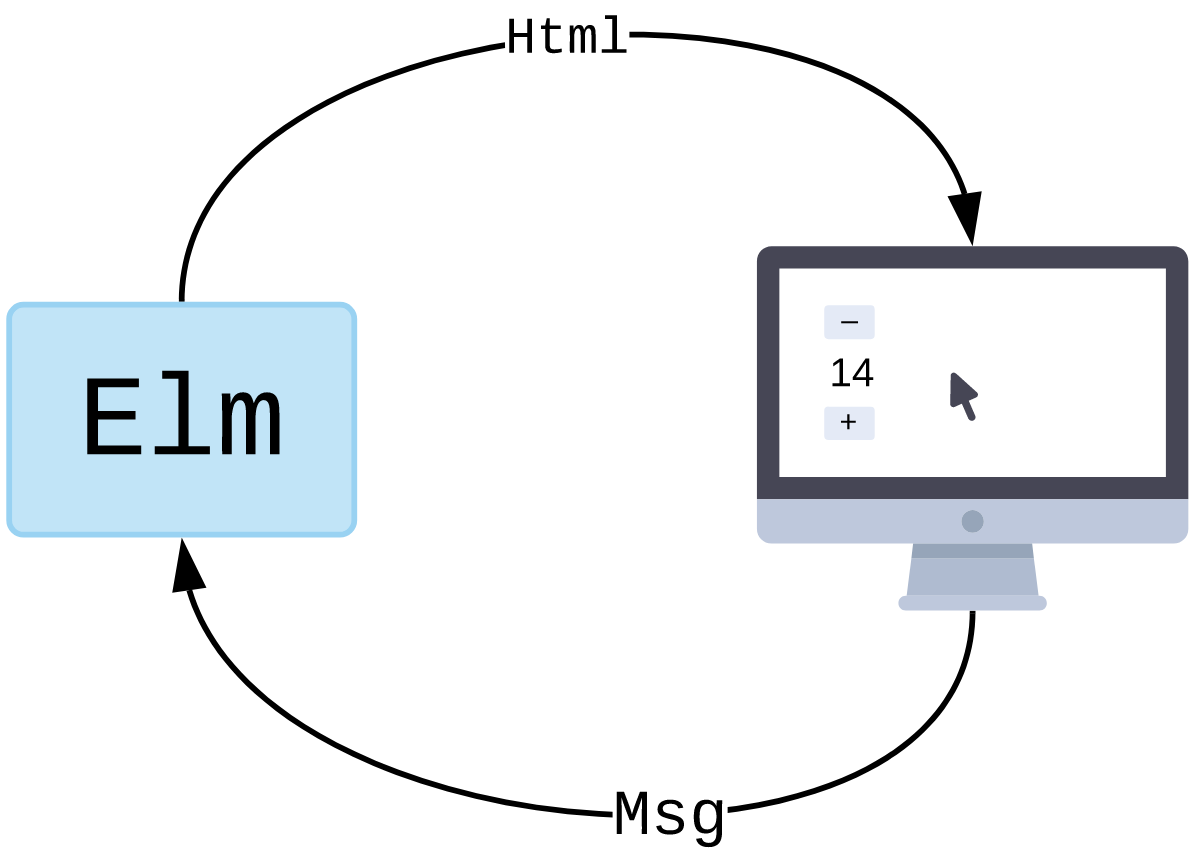
\includegraphics[width=0.6\textwidth]{elm_arch.png}
    \caption{The Elm Architecture}
    \label{fig:elm_arch}
\end{figure}

Architektura Elma składa się z trzech podstawowych elementów:
\begin{itemize}
    \setlength\itemsep{-0.1em}
    \item Model -- opisujący stan aplikacji
    \item Update -- opisujący logikę aplikacji
    \item View -- opisujący wygląd aplikacji
\end{itemize}


\subsection{Model}
\begin{minipage}{.55\textwidth}
Celem modelu jest zdefiniowanie danych w naszej aplikacji. W tym przypadku model będzie bardzo prosty - jedna wartość liczbowa, która może zostać zwiększona lub zmniejszona.
\end{minipage}\hfill
\begin{minipage}{.35\textwidth}
\lstset{frame=single}
\begin{lstlisting}[caption={Model},label=kod:Model]
type alias Model = Int


init : Model
init =
  0
\end{lstlisting}
\end{minipage}\hfill

\subsection{Update}
\begin{minipage}{.45\textwidth}
\lstset{frame=single}
\begin{lstlisting}[caption={Update},label=kod:Update]
type Msg
  = Increment
  | Decrement


update : Msg -> Model -> Model
update msg model =
  case msg of
    Increment ->
      model + 1

    Decrement ->
      model - 1
\end{lstlisting}
\end{minipage}\hfill
\begin{minipage}{.45\textwidth}
Funkcja update ma za zadanie opisywać jak nasz model będzie się zmieniał w czasie. Może odebrać dwa typy wiadomości - Increment i Decrement. W wyniku operacji update otrzymujemy nowy, zaktualizowany model.
\end{minipage}\hfill
\subsection{View}
Funkcja view jako argument przyjmuje model i zwraca kod HTML. Wykorzystany został tutaj handler onClick, który po kliknięciu generuje odpowiednią wiadomość. Znak plusa generuje wiadomość Increment, znak minusa Decrement. Wybrana wiadomość trafia do funkcji update.

\lstset{frame=single}
\begin{lstlisting}[caption={View},label=kod:View]
view : Model -> Html Msg
view model =
  div []
    [ button [ onClick Decrement ] [ text "-" ]
    , div [] [ text (String.fromInt model) ]
    , button [ onClick Increment ] [ text "+" ]
    ]
\end{lstlisting}


% --------------------------------------------------------------------------------
\chapter{Instrukcja laboratoryjna}
W poniższym rozdziale przedstawiam przykładową instrukcję laboratoryjną, która krok po kroku przeprowadza czytelnika przez proces tworzenia aplikacji w Elmie, zaczynając od przygotowania środowiska deweloperskiego, przez podstawy języka wraz z ćwiczeniami pozwalającymi na lepsze zrozumienie składni, aż po stworzenie większej aplikacji frontendowej.

\section{Instalacja środowiska}
\subsection{Linux}
\subsection{Windows}

\section{Podstawy języka Elm}

\section{Aplikacja frontendowa}

% --------------------------------------------------------------------------------
\chapter{Podsumowanie}


% --------------------------------------------------------------------------------
\backmatter

% lista rysunków
\listoffigures
% lista tabel
\listoftables
% lista algorytmów
\listofalgorithms

% rodzaj bibliografii
\bibliographystyle{plain}
% plik z wpisami bibliograficznymi
\bibliography{bibliografia}
\end{document}
